\documentclass{article}

\usepackage{graphicx}
\usepackage{multicol}
\usepackage{fullpage}
\usepackage{floatflt}

\def\deg{$^{\circ}$ }
\def\degf{$^{\circ}$F }
\def\ms{m~s$^{-1}$}
\def\sec{s$^{-1}$}
\def\hr{h$^{-1}$}
\def\etal{{\it et al.}, $\;\;$}
\def\jas{{\it J. Atmos. Sci.}, $\;\;$}
\def\wf{{\it Wea. Forecasting}, $\;\;$}
\def\vol #1 {{\bf #1}, $\;\;$}
\def\refer{\par\noindent\hangindent\parindent\hangafter1}


\title{Herzmann Family Christmas Letter 2013}
\author{Daryl Herzmann${}^1$, Elizabeth Herzmann${}^1$, AND Margaret Herzmann${}^2$ \\
\it{${}^1$ Caretakers},
\it{${}^2$ Precious Baby}} 
\date{07 December 2013}

\makeatletter
\newenvironment{tablehere}
  {\def\@captype{table}}
  {}

\newenvironment{figurehere}
  {\def\@captype{figure}}
  {}
\makeatother

\newcommand{\Line}[0]{%
  \rule{0cm}{0cm}\\\hrule\rule{0cm}{0cm}%
}

\begin{document}
\maketitle

\begin{abstract}
Occurring on a date so close to the start of the New Year, it follows that
the Christmas Letter summaries a year's worth of activities for our family.
During the past year, we were able to increase the size of our family by
50\% (33\% if you include our cat) and increase the baby production rate
when measured from our date of marriage.  During these activities, both
caretakers were able to maintain their employment status and complete other
necessary tasks for survival.  At this time, the entire family is healthy
and are productive members of society.

\end{abstract}

\Line

\begin{multicols}{2}

\section{Introduction}
Our family conists of four functioning units:  Daryl [35] the loving
husband, Liz [29] the caring wife, Margaret (Miss Maggie hereafter) [0] 
the happy baby, and Snoopy [6] the tempormental cat.  The combined output
of our family is presented in this arcticle with key events summarized in
table~\ref{timeline}.

\subsection{Housing}

We continue to make our residence in the fine suburb of Des Moines 
named Ankeny.  The reader may recall Daryl and Liz living on the
Iowa State University Agronomy Farm.  While a nice location and free,
if was not large enough to sustain family expansion and so we moved 
in May 2012 to a much larger facility here in Ankeny.  Our current home 
was built in 1996, consisting of three levels, a two car garage, and
four bedrooms.  Daryl vowed to the realitor that our family would never
move from this location.  We advise that it is safe to write our mailing
address in your address book with an ink pen.

\subsection{Conveyances}

Our family has three means of transporation at this time.  A 2008 Pontiac 
Vibe, which has a manual transmission that only Daryl can drive.  A 2012 
Honda Fit, which gets great gas mileage and served us well for a trip to
Dallas this past summer.  We also have one bicycle with a single seat.
None of these appear to be well suited for a growing family, so consideration
has been made to purchasing a minivan.  At this time, Daryl, as the fiduciary,
has yet to approve of the request.

\begin{figurehere}
 \centering   
 \resizebox{.95\columnwidth}{!}{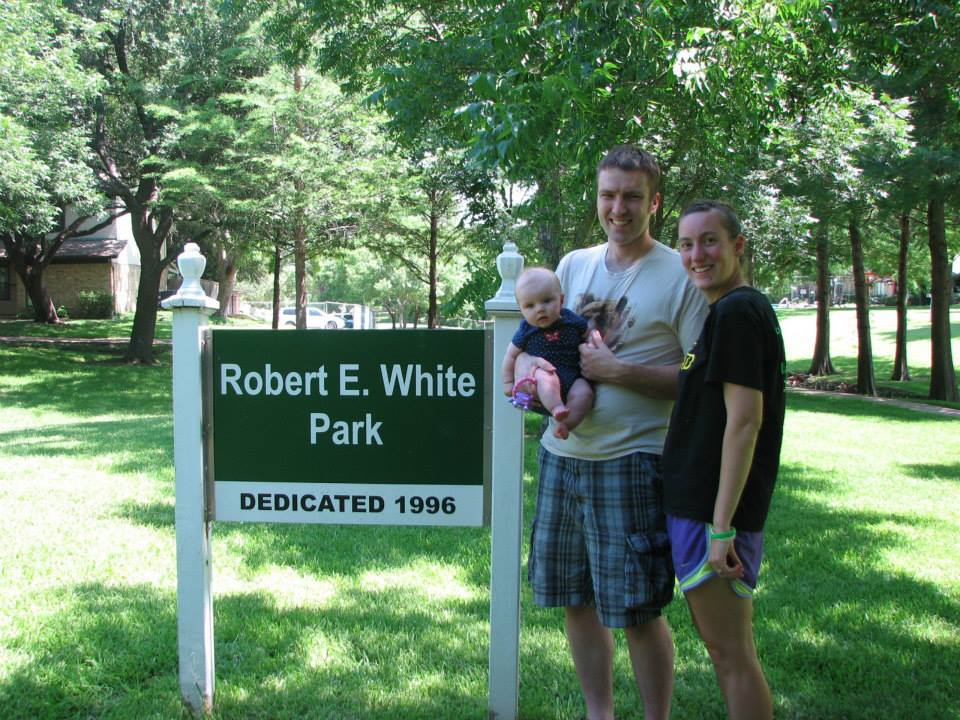
\includegraphics[angle=0]{plots/park.ps}}
 \caption{From left to right: Miss Maggie, Daryl, and Liz visiting the park
in Dallas named after Liz's grandfather.}
\end{figurehere}

\subsection{Employment}

Liz returned to working with the students at Johnston Middle School for the
4th year.  Her teaching duties include half time 9th grade Physical Science
and half time 8th grade Advanced Science.  She is looking forward to having
a student teacher in the spring and getting to teach in a new way.  She
also helps out after school with the Science Olympiad teams which will
compete in March.  Last spring, she had the opportunity to coach the 8th
grade girls track team, but will not be coaching this year.


\begin{table*}[t]
 \begin{center}
  \begin{tabular}{|c|c}
   \multicolumn{1}{c}{Date} &
   \multicolumn{1}{c}{Event} \\ \hline \hline
   13 January     & Miss Maggie was born! \\
  \end{tabular}
 \end{center}
 \caption{Important events for our family during 2013.}
 \label{timeline}
\end{table*}


\section{Miss Maggie}

As the Psalmist King David writes: "Children are a hertitage from the Lord"
and thus we have been so blessed with our new addition this year.  She was born on
a cold Sunday morning (13 January) after a relatively easy delivery (as 
characterized by Daryl).  Our delivery story began around 00 LST and was 
completed some nine hours later.

\section{Trip to Dallas}

\section{Baby Number Two}

\section{Summary}

\bigskip
  \emph{Acknowledgments} Our family wishes to thank you for the generous 
support, prayers, cards, gifts, and visits you have provided us in the past
year.

\section{References}

\refer King David, ~700 BC: Psalm 127: 3-5 \vol 1.

\end{multicols}

\end{document}

